\section{Application: \\
Revealing ISP Behavior}
\label{sec:isp-behavior}

This section describes how we build two applications atop \meddle to 
reveal the policies ISPs apply to mobile traffic traversing their networks. 
Previous work focused on addressing this problem in fixed-line networks; to 
the best of our knowledge we are the first to provide this functionality for 
mobile systems.

\subsection{Detecting Content Manipulation}

ISPs, middleboxes and client software are known to change Web page content for 
a variety of reasons including performance optimization and security. In some cases, 
a third party can change a page for selfish reasons, \eg to insert ads that generate revenue 
for that party. Figure~\ref{fig:tripnet-example} depicts an example of content injection in China, where 
a banner ad is replaced by information about the local airport.

\begin{figure}
\centering
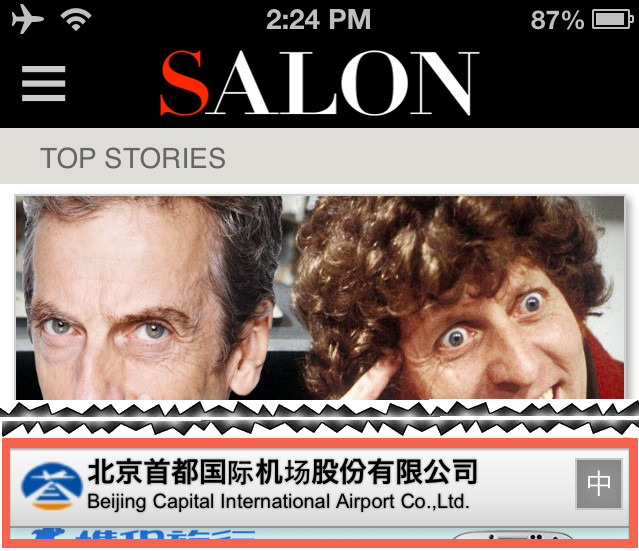
\includegraphics[width=0.8\linewidth]{figures/injectioncrop.png}
\caption{\textbf{Screen capture of content injection by a Chinese ISP in November, 2013.} \emph{The 
highlighted region at the bottom should be an advertisement from a US company.} }
\vspace{\postfigspace}
\label{fig:tripnet-example}
\end{figure}


This problem of Web interference was first highlighted by Reis~\etal~\cite{reis:tripwires}. 
The authors demonstrated that although a small percent of users were affected by in-flight changes, those changes tend to introduce vulnerabilities including cross-site scripting (XSS) attacks. 
They proposed and deployed \emph{Web Tripwires}, Javascript code to detect in-flight page changes. 
The main limitation of \emph{Web Tripwires} is that it requires each Web site to modify their content to include a tripwire.

In \meddle, we extended tripwires to alleviate this limitation. 
Namely, we use the HTTP proxy present in \meddle to inject a tripwire on \emph{any} page 
without requiring support from Web site developers -- an approach we call a \emph{Web Tripnet}.

\noindent\textbf{Implementation.} With \meddle all traffic is tunneled, thereby 
preventing ISPs from modifying pages. To identify ISP content manipulation 
(\eg for public policy reasons and for users not protected by \meddle), we provide the Tripnet as an opt-in feature. Because this entails 
two fetches of every Web page, we also support two modes: always-on and low-rate random trials, where we 
insert tripwires for some small fraction of their visited sites.

The Tripnet works as follows (Fig.~\ref{fig:tripnet}). A client requests a Web page through the \meddle VPN 
tunnel. This request is forwarded to the destination server. The response returns to 
the \meddle server, where a transparent proxy injects the tripwire code.\footnote{We 
recognize the irony of injecting content to detect content injection, but this is done only with user consent.}
The tripwire-enabled response is forwarded to the client, which executes the Javascript at page load time.


\begin{figure}
\centering
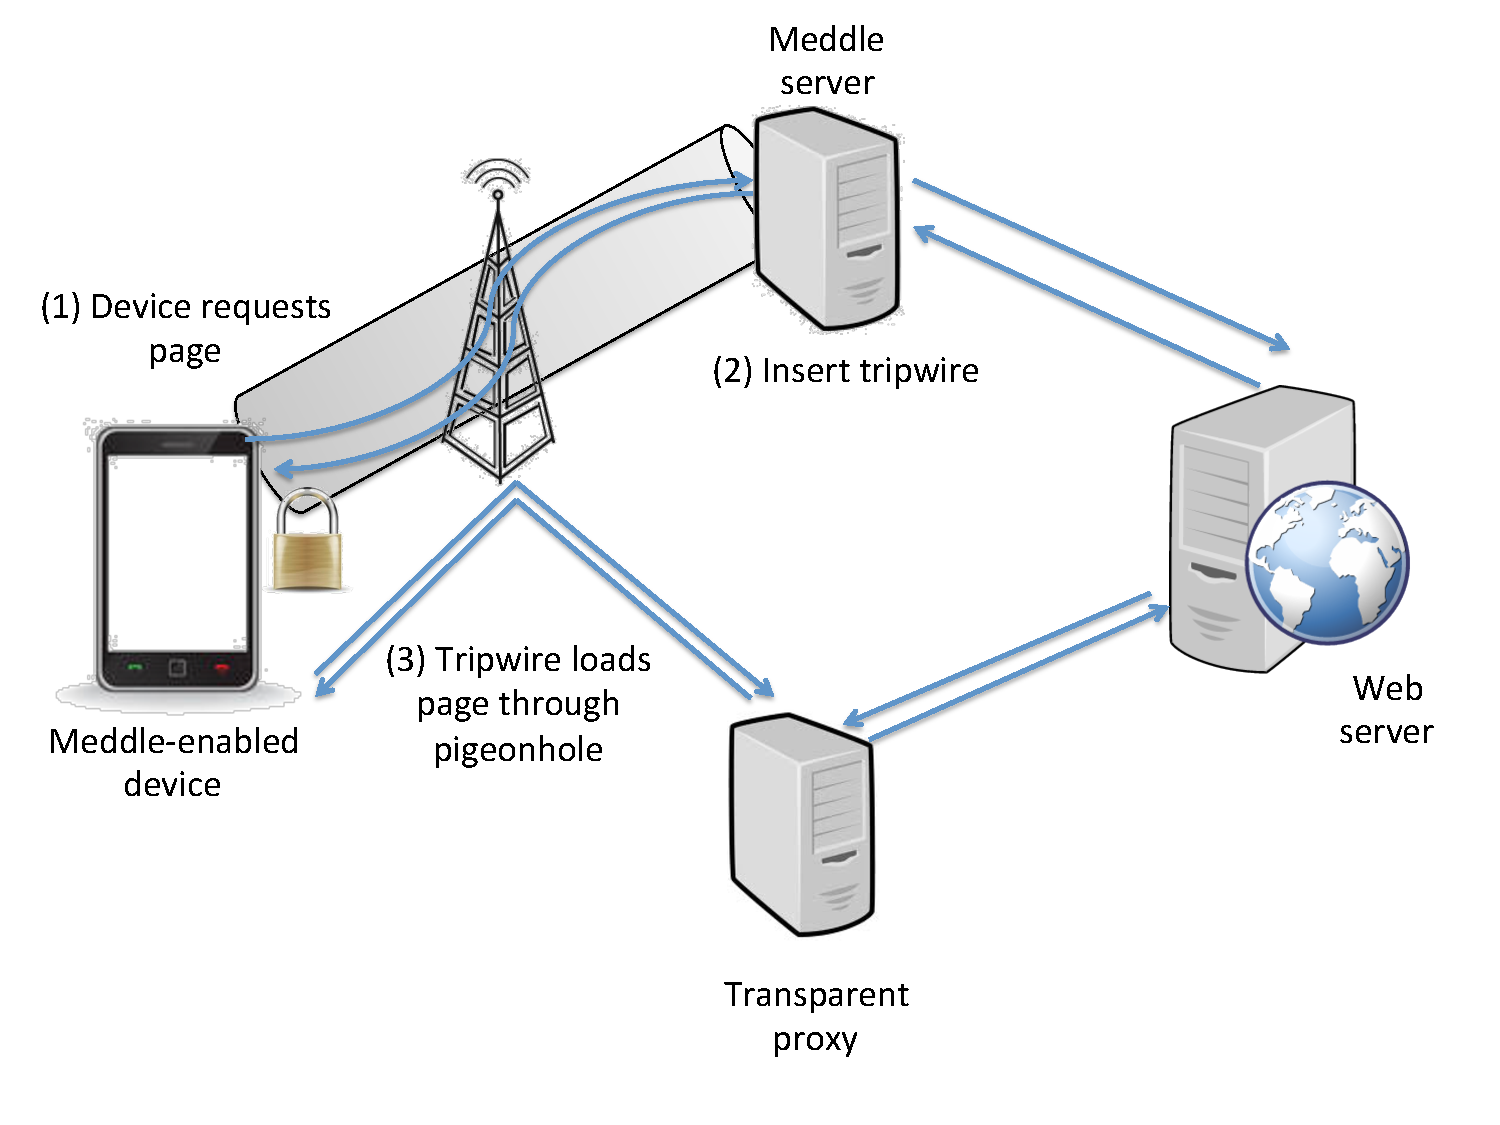
\includegraphics[width=0.9\linewidth]{figures/tripnet.pdf}
\vspace{-1em}
\caption{\textbf{Overview of the Web Tripnet.} \emph{A Web page loads 
through the VPN tunnel, where a \meddlebox inserts a Web tripwire. The
tripwire causes the browser to reload the Web page using the address of a
transparent proxy server that is accessed using an unencrypted connection.
After the proxied version of the page is loaded, the browser (or a \meddlebox)
compare the two pages to identify manipulation.} }
\label{fig:tripnet}
\vspace{\postfigspace}
\vspace{-1em}
\end{figure}

The tripwire code contains information about the page content prior to traversing the ISP. When 
executed, the code fetches the page again to compare with the (known) unmodified page content.  
To ensure that this fetch does \emph{not} traverse the VPN connection, we use a \emph{pigeonhole} domain 
whose traffic traverses an untunneled interface. For example, if the original request was for \url{www.facebook.com}, 
we send the request to \url{tripnet.meddle.mobi/www.facebook.com}, where we run a Web proxy. 

When the request arrives at our proxy server, we could forward the request to the original target. In 
practice, however, doing so would return different content due to the highly dynamic nature of most 
Web content. Instead, we cache Web pages at the tripnet-injecting server and co-locate our Web proxy 
there. Thus we return exactly the same Web page that was received over the tunneled connection. 
Any difference in page content can only be due to ISP behavior. 

Note that this does not address cases 
where modification is based on destination IP or when the entire page is replaced (\eg a block page). 
To detect this, we can set the tripwire to fetch the page from the origin server at the cost of imprecise 
identification due to dynamic content.  

\noindent\textbf{Content modification/replacement.}
In addition to detecting changes to text content in 
Web pages, we use our controlled experiments to investigate whether ISPs are manipulating 
media content, \eg downsampling high-resolution images to reduce bandwidth consumption 
from mobile devices. For this experiment, we augment our Tripnet experiments with the result 
of wget results from the mobile device and the proxy server. Note that this experiment requires an 
app or tethered laptop to collect the Web media objects fetched over the mobile network.

\noindent\textbf{Sites and ISPs tested.} We conducted controlled experiments using our Tripnet 
architecture, using the top 100 Web sites according to Alexa. We tested using 
AT\&T, T-Mobile and Verizon in the US, and Sosh in France. 
Many sites customize content according to \useragent strings, so we spoof them  
as coming from iOS, Android and desktop clients.



\noindent\textbf{Content modification/injection.} We found no cases of page modifications in 
the networks tested. In addition the example in Fig.~\ref{fig:tripnet-example}, we found whole-page replacement in the case of T-Mobile. A 
service called \emph{Web Guard} replaced the page for an adult Web site with a block page. 
Further, our tests allowed us to identify differences in Web content not due an ISP. Specifically, 
we observe that Wordpress hosts a jquery.js file using the Edgecast CDN, and the file contents 
differ depending on where the client is located. When accessed directly from mobile devices the 
script size is 256\,KB; when accessed from the proxy server the script is 93\,KB. The difference in 
size is because the latter uses a minified version; it is unclear why this is not served 
to all the networks.

\subsection{Detecting Service Differentiation}

In this section, we describe how we use \meddle to detect service differentiation 
in ISPs. 
%To the best of our knowledge, this is the first system to provide such information 
%in mobile systems.
%
We define service differentiation as any attempt to change the performance 
of network traffic traversing an ISP's boundaries. ISPs may implement differentiation policies 
for a number of reasons, including load balancing, bandwidth management or business reasons. 
Specifically, we focus on detecting whether certain types of network traffic receive 
better (or worse) performance. 

Previous work~\cite{dischinger:glasnost,tariq:nano,zhang:netdiff} explored this problem in limited 
environments. Glasnost focused on BitTorrent in the desktop/laptop environment, 
and lacked the ability to conduct controlled experiments to provide strong evidence 
of differentiation. NetDiff covered a wide range of passively gathered traffic from a 
large ISP but likewise did not support targeted, controlled experiments. We now 
describe how we address these limitations with \emph{Mobile Replay}. 

\noindent\textbf{Assumptions.} We assume that ISPs will differentiate traffic based on hostname, 
IP addresses, ports, total number of connections, payload signatures, total bandwidth and time of day. 
Our system can diagnose nearly all of these cases. 

\noindent\textbf{Overview.} Mobile Replay identifies service differentiation using 
two key components. First, it tests for differentiation by replaying real network traces 
generated from user interactions with apps. \meddle facilitates capturing this information, 
and we develop new strategies for replaying arbitrary app traces. Second, Mobile 
Replay exploits the \meddle VPN to conduct controlled experiments. By alternately replaying 
traffic over tunneled and untunneled connections multiple times in rapid succession, we control 
for factors that ISPs may use to differentiate traffic.

\begin{table*}[ht]
\begin{center}
{\footnotesize
\begin{tabular}{|l|l|l|l|l|l|}
\hline
 & \textbf{Network Coverage} &  \textbf{Portability} &  \textbf{Deployment model} &   \textbf{Meas. Type}  & \textbf{Control?} \\ \hline
Large ISP studies~\cite{vallina-rod:ads,gerber:passivespeed} & Single carrier & All OSes & Instrument cell infrastructure & Passive & No \\ \hline
WiFi study~\cite{chen:wifi} & Single WiFi network & All OSes & Instrument WiFi network & Passive & No \\ \hline
PhoneLab~\cite{PhoneLab}/TaintDroid~\cite{enck:taintdroid} & Multiple networks & Android & Install custom OS & Active/Passive & Yes \\ \hline
MobiPerf~\cite{wang:middleboxes}/SpeedTest~\cite{sommers:cellwifi} & Multiple networks & Android & Install App & Active & Yes \\ \hline \hline
\platname & Any network & Most OSes & VPN configuration & Active/Passive & Yes \\ \hline
\end{tabular} }
\end{center}
\vspace{\postfigspace}
\caption{\textbf{Comparison of related work.} \emph{ \platname is the first approach to provide visibility and control over network traffic for all access 
networks and most device OSes}.}
\label{tab:relatedCompare}
\vspace{\postfigspace}
\end{table*}%

A key challenge is how to capture and replay 
the salient features of application traffic such that it will be subject to differentiation 
from middleboxes. To this end, we design a system that captures 
traffic generated by users' devices (via \meddle) and replays those flows 
from a \emph{replay server}. 

The replay system consists of a client running on the mobile device and a replay server. 
The client and server coordinate to replay the original flows in a way that reproduces packet timings, 
sequence of bytes, ports and source IPs. Since our replay is limited to using our own replay servers,
 we cannot detect differentiation based on arbitrary destination IPs. \drc{Add UDP challenges?}


\begin{figure}
\centering
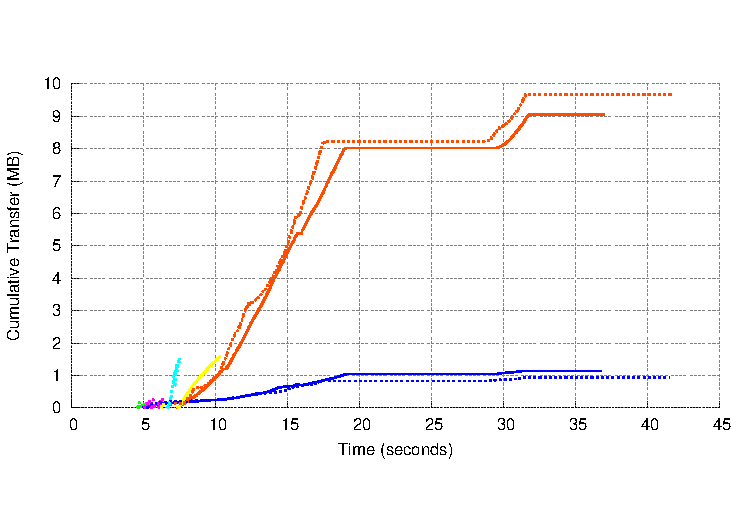
\includegraphics[width=0.9\linewidth]{plots/netflix_seqnum_wifi_vs_cell.pdf}
\caption{\textbf{Plot of record (solid) and and replay (dashed) from Netflix activity.} \emph{The x-axis is time and y-axis is the 
total number of bytes transferred to that point. The figure shows that our replay closely matches 
the recorded trace.}}
\vspace{\postfigspace}
\label{fig:replaySimilarity}
\end{figure}

Another key challenge is how to establish ground truth as to whether the ISP is 
differentiating service for replay traffic. To address this, we exploit the VPN connection 
that \meddle provides as follows. When the 
VPN is enabled, the ISP cannot inspect flow contents and thus cannot differentiate based 
on the above factors except total bandwidth and time of day. 
We then compare this performance to the case when we send traffic untunneled.  
Using multiple successive trials of tunneled and untunneled replay experiments, 
we can determine the noise inherent in performance metrics in each type of experiment (tunneled vs not tunneled), then 
identify cases where there are statistically significant differences between 
them -- indicating differentiation. 

%Overview of the approach and challenges. \meddle allows us to capture 
%traces from mobile devices over both \wifi and cell, meaning we can model 
%behavior from either medium. \meddle also serves as a convenient location 
%to conduct replay experiments. The challenge is how to capture and replay 
%the salient features of application traffic such that it will be subject to differentiation 
%from middleboxes. State what we can reproduce (timings, sequence of bytes, ports and source IPs) 
%and what we cannot (destination IPs from client). Challenges with UDP. Challenges 
%with different network conditions. Differences from Glasnost.




\noindent\textbf{Feasibility.}
Figure~\ref{fig:replaySimilarity} uses a sequence-number diagram to compare the behavior of original traces 
to those generated by our replay system, in an environment where we know differentiation is not happening. 
By preserving packet ordering and timing, our system produces very similar results. 


Of course, a variety of factors can differ between record and replay, including network 
conditions and access technology. In particular, apps may change their behavior in response 
to network technology and available bandwidth. For example, the YouTube app does not 
allow HD video content over cellular networks. In such cases, we must ensure that we replay 
traffic that was originally captured over similar network conditions. 
In our experiments, YouTube was the only app that exhibited such behavior.


%\textbf{Graph}: If we find a case of difference between \wifi and cell, plot it here.



\noindent\textbf{Methodology.} We detect differentiation according to the following metrics. First, we 
compute checksums to verify that the bytes sent/received at each endpoint during the replay are 
exactly the same as the original trace. If not, we flag a case of content manipulation/blocking. Second, we
compute summary statistics on throughput, latency and loss. Unlike manipulation/blocking, there are 
confounding factors other than differentiation that may causes changes in these statistics between the 
record and replay.

To address this issue, we run multiple replay trial (10 total), alternating between using a VPN connection ($R_T$) and 
an untunneled one ($R_U$). By computing statistics over multiple trials of one category ($R_T$ or $R_U$) we can quantify 
natural variations in performance that are not a result of differentiation. Having computed the variance over $R_T$ and $R_U$, we can 
compare the summary statistics (mean/median) of $R_T$ and $R_U$ and use the variance in each category 
to determine if the differences are statistically significant.

Note that ISPs may apply differentiation to all VPN traffic, \eg by throttling. To detect this, we group all $R_T$ 
samples and compare them to all $R_U$ samples across all applications and use the analysis described above. 

%\textbf{Graph}: Similarity score for network traffic in setting where we know there is no differentiation. 
%Score can include overall throughput, latency characteristics, loss, packet timings.

\noindent\textbf{Results from wide-area testing.} We used Mobile Replay to investigate service differentiation in 
AT\&T, Verizon, and T-Mobile, using the following apps: YouTube, Netflix, Spotify and Dropbox. 
We picked these apps because they are popular and bandwidth-intensive, and thus are potential candidates 
for differentiation due to traffic engineering. We interact with these apps for about one minute during the record 
phase, then replay the traces in each measured network. Note that these apps are intended to demonstrate 
how our approach works; a complete treatment of service differentiation is beyond the scope of this paper. 

Table~\ref{} shows our results for throughput, loss and RTT.     
 
\textbf{Table}: each row is an app, each column is the average values and stddev for performance. I suppose 
this will clearly show that ISPs are not differentiating.
 

%\textbf{Table}: each row is an app, each column is an ISP, each cell is a marker indicating what kind of 
%differentiation is happening
%
%\textbf{Graph}: Plot showing a sequence of traces that demonstrates what this differentiation looks like


